Arranjo é uma denominação utilizada para uma permutação de \textbf{\textit{n}} objetos tomados \textbf{\textit{r}} a \textbf{\textit{r}}, com \textbf{\textit{r}} \textit{menor} do que \textbf{\textit{n}} (\textbf{\textit{r}} $\leq$ \textbf{\textit{n}}), ou seja, é uma escolha de \textbf{\textit{r}} entre esses \textbf{\textit{n}} objetos na qual a ordem importa.

Para obter uma fórmula para A(n,r), temos \textbf{\textit{r}} diferentes espaços onde os \textbf{\textit{n}} objetos podem ser colocados.

\begin{figure}[H]
	\centering

	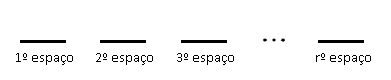
\includegraphics[width=7cm]{C:/Users/Andressa-PC/Desktop/estatistica/esqueleto/imagens/arranjo_demo.png}

\end{figure}

Assim, A(n,r) pode ser considerado a quantidade de maneiras de colocar \textbf{\textit{n}} objetos distintos em \textbf{\textit{r}} espaços.

Supondo primeiramente que o número de objetos é igual ao número de espaços (\textbf{\textit{n}}=\textbf{\textit{r}}), teríamos n objetos para ocupar o primeiro espaço, n-1 para o segundo, n-3 para o terceiro e assim por diante, de forma que ao chegar no último espaço teremos apenas um objeto para escolher.
Logo, pelo princípio fundamental da contagem descrito anteriormente temos
\begin{center}
	$A(n,n)=n\ \ .\ \ (n-1)\ \ .\ \ (n-2)\ \ .\ \ (n-3)\ \ ...\ \ 1$
	
ou

	$A(n,n)=n!$
\end{center}

\noindent 
Por exemplo, 
\begin{center}
	$A(4,4)= 4\ \ .\ \ 3\ \ .\ \ 2\ \ .\ \ 1\ \ =\ \ 4!$
\end{center}
Isso também pode ser aplicado para um A(n,r), ou seja, para o caso em que o número de espaços é menor que o número de objetos. Por exemplo,
\begin{center}
	$A(10,4)= 10\ \ .\ \ 9\ \ .\ \ 8\ \ .\ \ 7$
\end{center}
Generalizando, podemos dizer que
\begin{center}
	$A(n,r)\ \ =\ \ n\ \ .\ \ (n-1)\ \ .\ \ (n-2)\ \ .\ \ (n-3),...,(n-(r-1))$

ou

	$A(n,r)\ \ =\ \ n\ \ .\ \ (n-1)\ \ .\ \ (n-2)\ \ .\ \ (n-3)\ \ ...\ \ (n-r+1)$
\end{center}

\noindent
multiplicando por $\frac{(n-r)!}{(n-r)!}$, podemos reescrever A(n,r) como\\

$A(n,r)\ \ =\ \ n\ \ .\ \ (n-1)\ \ .\ \ (n-2)\ \ .\ \ (n-3)\ \ ...\ \ (n-r+1)\ \ .\ \ \frac{(n-r)!}{(n-r)!}$

\hspace{\parindent}
$=\ \ \frac{n\ \ .\ \ (n-1)\ \ .\ \ (n-2)\ \ .\ \ (n-3)\ \ ...\ \ (n-r+1)\ \ .\ \ (n-r)!}{(n-r)!}$ 

\hspace{\parindent}
$=\ \ \frac{n\ \ .\ \ (n-1)\ \ .\ \ (n-2)\ \ .\ \ (n-3)\ \ ...\ \ (n-r+1)\ \ .\ \ (n-r)\ \ ...\ \ 3\ \ . \ \ 2 \ \ . \ \ 1}{(n-r)!}$ 

\hspace{\parindent}
$=\ \ \frac{n!}{(n-r)!}$\\

\noindent
pois, como descrito anteriormente, sabemos que no fatorial vamos subtraindo uma unidade de n até alcançar o 1

\begin{center}
	$n!\ \ =\ \ n\ \ .\ \ (n-1)\ \ .\ \ (n-2)\ \ .\ \ (n-3)\ \ ...\ \ (n-r+1)\ \ .\ \ (n-r)\ \ ...\ \ 3\ \ . \ \ 2 \ \ . \ \ 1$
\end{center}

\noindent
Dessa forma, chegamos a fórmula de arranjo
\begin{equation}
A(n,r) = \frac{n!}{(n-r)!}
\end{equation}

\noindent
Exemplo 1: Em certo país as placas dos automóveis tem letras, e não números,que as distinguem. Precisamente quatro letras são usadas. Quantas placas podem ser feitas se contamos com um alfabeto de 26 letras? E se não fosse permitido usar letras repetidas em uma placa?

Para a primeira letra da placa teremos 26 opções, para a segunda também teremos 26 opções, e assim por diante. Se há 4 posições possíveis para alocar essas letras, então teremos $26^4$ possibilidades de escolha.

Se não utilizarmos letras repetidas, ficamos com 26.25.24.23 ou  $\frac{26!}{22!}$ possibilidades de escolha\\

\noindent
Exemplo 2: Quantos inteiros entre 100 e 999 consistem de dígitos ímpares distintos?

Os dígitos ímpares são 1, 3, 5, 7 e 9, logo n=5. Além disso, os número serão formados por 3 dígitos, logo r=3. Assim podemos dizer que vamos realizar uma permutação de 5 objetos tomados 3 a 3, ou seja, A(5,3).

\begin{center}
	$A(5,3) = \frac{5!}{(5-3)!}= \frac{5!}{2!}=\frac{5.4.3.2!}{2!}=5.4.3=60 \ \ inteiros$
\end{center}


